\documentclass{article}

\usepackage{graphicx}
\usepackage{tikz}
\usepackage{tikzsymbols}
\usetikzlibrary{calc,patterns,shapes.geometric}
\pagestyle{empty}
\usepackage[margin=0pt]{geometry}
\geometry{papersize={14in,12in}}

\def\centerarc[#1](#2)(#3:#4:#5){\draw[#1] ($(#2)+({#5*cos(#3)},{#5*sin(#3)})$) arc (#3:#4:#5);}

\begin{document}
	\begin{figure}
		\centering
		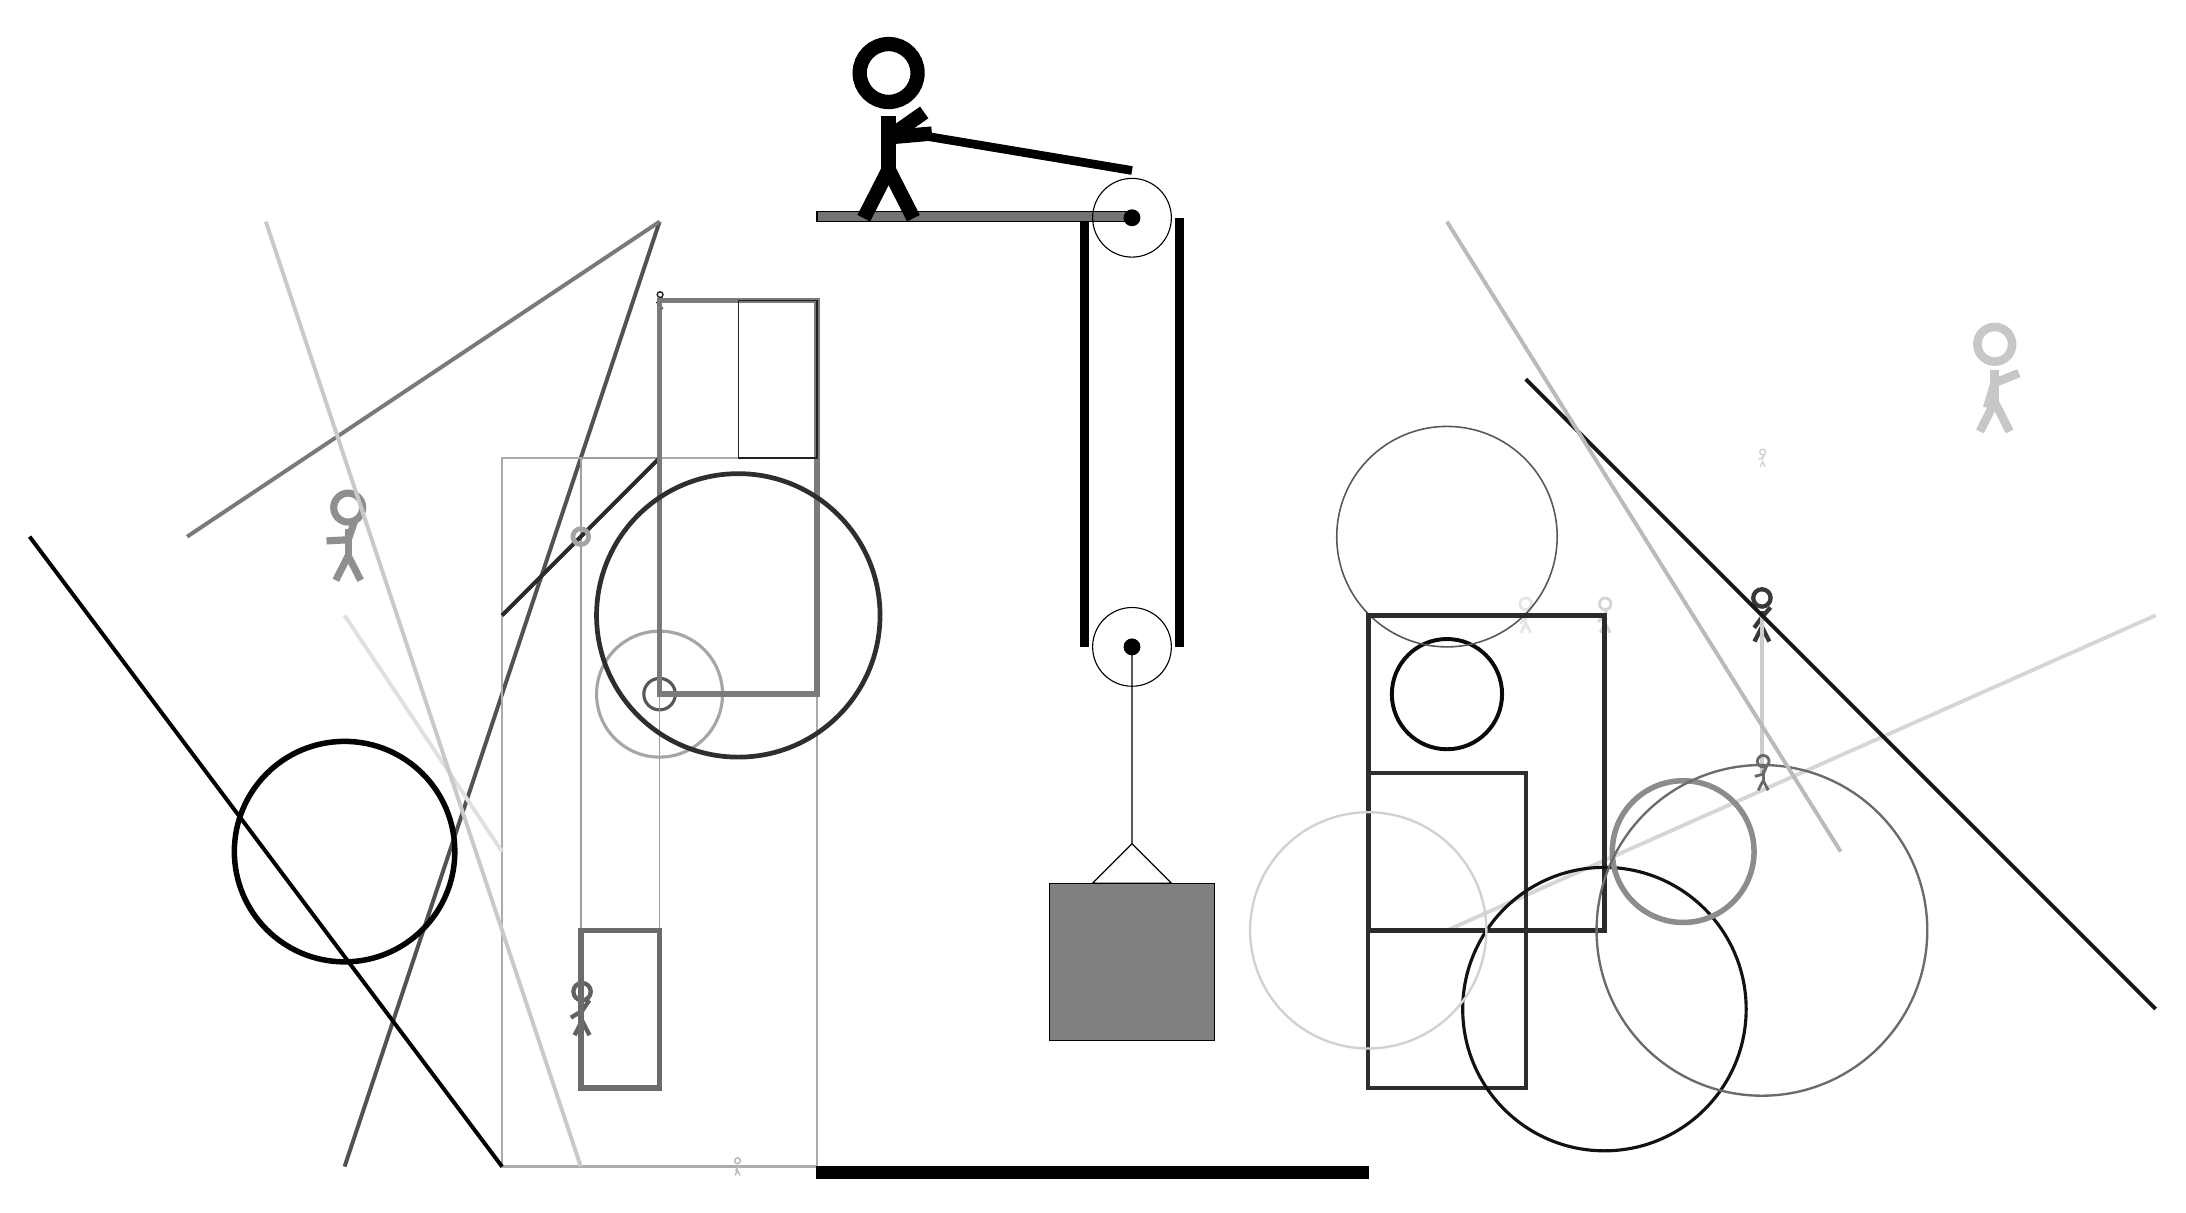
\begin{tikzpicture}
			%%%%% START %%%%%
			
			\draw[fill=black!55] (-2, 9) rectangle (2, 9.125);
			
			\draw (2, 3.6) circle (0.5);
			\draw[fill=black] (2, 3.6) circle (0.1);
			
			\draw (2, 9.05) circle (0.5);
			\draw[fill=black] (2, 9.05) circle (0.1);
			
			\node[line width=0.2mm, color=black!62] at (-5, -1) {\Strichmaxerl[3][31][56]};
			
			\draw[line width=0.5mm, color=black!68](-4, 9) -- (-8, -3);
			\node[line width=0.3mm, color=black!17] at (8, 4) {\Strichmaxerl[2][33][82]};
			\node[line width=0.2mm, color=black!18] at (10, 6) {\Strichmaxerl[1][3][64]};
			
			\node[line width=0.3mm, color=black!10] at (7, 4) {\Strichmaxerl[2][54][54]};
			
			\draw[line width=0.3mm, color=black!33] (-2, 6) rectangle (-6, -3);
			
			\node[line width=0.2mm, color=black!85] at (-4, 8) {\Strichmaxerl[1][23][63]};
			
			\draw [line width=0.4mm, color=black!66](-4, 3) circle (0.2);
			\draw [line width=0.5mm, color=black!96](6, 3) circle (0.7);
			
			\draw [line width=0.4mm, color=black!35](-4, 3) circle (0.8);
			\node[line width=0.5mm, color=black!78] at (10, 4) {\Strichmaxerl[3][54][49]};
			
			\draw[line width=0.5mm, color=black!100](-6, -3) -- (-12, 5);
			\draw[line width=0.5mm, color=black!16](6, 0) -- (15, 4);
			\draw[line width=0.2mm, color=black!38] (-4, -2) rectangle (-5, 6);
			\draw[line width=0.5mm, color=black!20](10, 4) -- (10, 2);
			\draw[line width=0.5mm, color=black!12](-6, 1) -- (-8, 4);
			
			\draw [line width=0.2mm, color=black!66](6, 5) circle (1.4);
			\draw[line width=0.6mm, color=black!83] (5, 0) rectangle (8, 4);
			\node[line width=0.2mm, color=black!28] at (-3, -3) {\Strichmaxerl[1][65][5]};
			
			\draw[line width=0.5mm, color=black!82] (5, -2) rectangle (7, 2);
			\draw [line width=0.4mm, color=black!93](8, -1) circle (1.8);
			
			\draw [line width=0.7mm, color=black!45](9, 1) circle (0.9);
			\draw [line width=0.7mm, color=black!99](-8, 1) circle (1.4);
			\draw[line width=0.5mm, color=black!83](-6, 4) -- (-4, 6);
			\node[line width=0.4mm, color=black!59] at (10, 2) {\Strichmaxerl[2][15][67]};
			
			\draw[line width=0.7mm, color=black!58] (-4, 0) rectangle (-5, -2);
			\draw[line width=0.7mm, color=black!52] (-2, 8) rectangle (-4, 3);
			\draw [line width=0.6mm, color=black!36](-5, 5) circle (0.1);
			\draw[line width=0.5mm, color=black!91](7, 7) -- (15, -1);
			\draw [line width=0.3mm, color=black!58](10, 0) circle (2.1);
			\draw[line width=0.5mm, color=black!52](-4, 9) -- (-10, 5);
			
			\node[line width=0.7mm, color=black!44] at (-8, 5) {\Strichmaxerl[5][3][71]};
			\draw [line width=0.3mm, color=black!18](5, 0) circle (1.5);
			\draw[line width=0.2mm, color=black!87] (-3, 8) rectangle (-2, 6);
			\node[line width=0.6mm, color=black!22] at (13, 7) {\Strichmaxerl[6][73][22]};
			\draw[line width=0.5mm, color=black!27](6, 9) -- (11, 1);
			\draw [line width=0.6mm, color=black!82](-3, 4) circle (1.8);
			
			\draw[line width=0.5mm, color=black!21](-5, -3) -- (-9, 9);
			
			\draw (2, 3.6) -- (2, 1.1) -- (1.5, 0.6) -- (2.5, 0.6) -- (2, 1.1);
			\draw[fill=black!50] (0.95, 0.6) rectangle (3.05, -1.4);
			
			\draw[line width=1.1mm] (1.4, 9) -- (1.4, 3.6);
			\centerarc[line width=1.1mm](2, 3.6)(180:360:0.6);
			\draw[line width=1.1mm](2.6, 3.6) -- (2.6, 9.05);
			\centerarc[line width=1.1mm](2, 9.05)(0:90:0.6);
			\draw[line width=1.1mm](2, 9.65) -- (-1, 10.15);
			
			\node at (-1, 10.15) {\Strichmaxerl[10][-175][35]};
			
			\draw[fill=black] (-2, -3) rectangle (5, -3.15);
			
			%%%%% END %%%%%
		\end{tikzpicture}
	\end{figure}	
\end{document}